\begin{surferPage}{双锥面}
    双锥面(右图)具有最简单的奇异点。它是唯一一个能够用二次多项式定义的奇异曲面:\[x^2+y^2-z^2=0.\]当把此等式右端的0用一个比较小的数$a\neq 0$替代后,双锥面变化为双曲面中的一种(由$a$的正负性决定):
    \begin{center}
      \begin{tabular}{@{}c@{\ }c@{\ }c@{\ }c@{\ }c@{}}
        \begin{tabular}{@{}c@{}}
          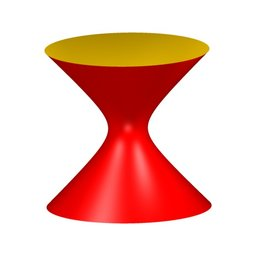
\includegraphics[width=1.2cm]{A1pm_2}
        \end{tabular}
        &
        $\leftarrow$
        &
        \begin{tabular}{@{}c@{}}
          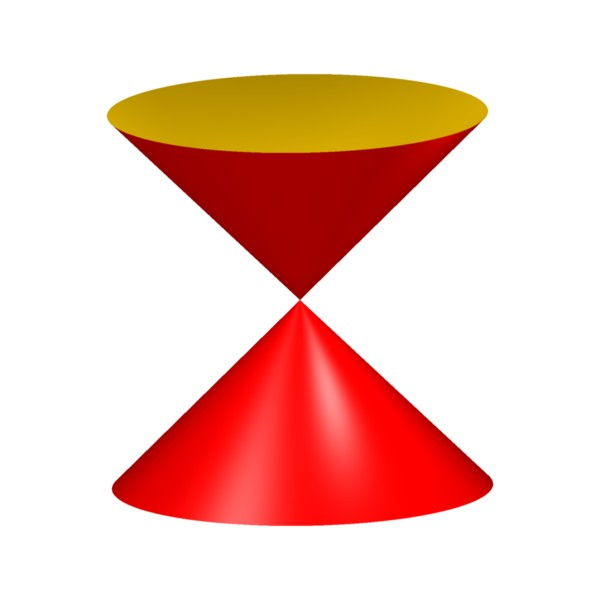
\includegraphics[width=1.2cm]{A1pm_1}
        \end{tabular}
        &
        $\rightarrow$
        &
        \begin{tabular}{@{}c@{}}
          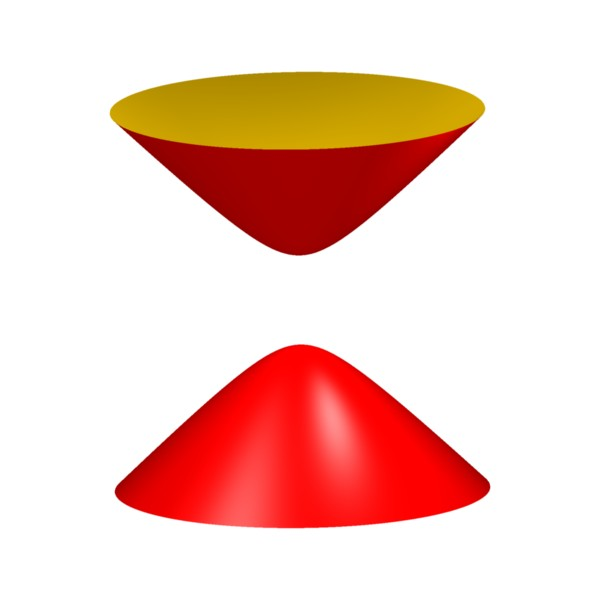
\includegraphics[width=1.2cm]{A1pm_0}
        \end{tabular}
      \end{tabular}
    \end{center}
   一个二次曲面的奇异点数不可能多于1,即$\mu(2)=1$。
\end{surferPage}
